\documentclass{article}
\usepackage{graphicx}
\usepackage{amsmath}
\usepackage{amsfonts}
\usepackage{amssymb}

\begin{document}

\title{ECE 110 Cramming Carnival Review}
\author{Author: Members of HKN}
\date{Fall 2024}
\maketitle

\section*{Introduction}
This worksheet does not cover content in lectures after November 25th and is not meant to be a replacement for any practice exams or section reviews. Use this worksheet as a quick refresher for various topics throughout the semester and for slightly different questions than the homeworks.

\section*{Formulas not on the help sheet}
\textbf{Note:} All formulas required for the questions are assumed to be known, as they are not provided in this sheet.
\begin{center}
    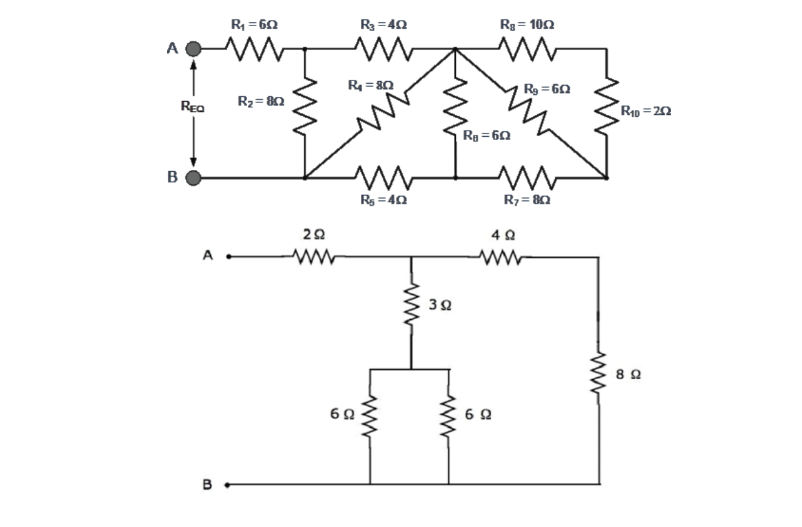
\includegraphics[width=0.75\linewidth]{figures/image.png}
\end{center}
\newpage

\section*{Power Efficiency \& Capacitors}
\textbf{Question 1:} Consider a car that has 400 kJ of energy at a specific speed. The car's regenerative brakes are 40\% efficient at converting kinetic energy to energy stored in a battery. What is the energy added when the car brakes to half speed?

\textbf{Solution:}
% Solution steps
\begin{align*}
    KE_{o} &= \frac{1}{2}mv^{2} \\
    KE_{\text{half}} &= \frac{1}{2} m {\left( \frac{v}{2} \right)}^{2}  = \frac{1}{2} m \cdot \frac{v^{2}}{4}  = \frac{1}{4} \cdot \frac{1}{2} m v^{2} =  \frac{1}{4} \times KE_{o} \\
    \Delta KE &= KE_{o} - KE_{half} = KE_{o} - \frac{1}{4}KE_{o} = \frac{3}{4}KE_{o} \\
    &= \frac{3}{4} \cdot 400kJ = 300 kJ \\
    E_{added} &= \%_{eff} \cdot \Delta KE = 0.40 \cdot 300kJ \\
    &= \boxed{120kJ}
\end{align*}

\textbf{Question 2:} If a 15 kWh battery has to be recharged using a 60\% efficient generator with peak power of 500 W, how long does the generator need to run to fully charge the battery?

\textbf{Question 3:} What is the energy stored in a 4 nF capacitor charged to 9V?

\textbf{Question 4:} What voltage is needed to charge the capacitor from the above question enough to lift a 2-gram mass 15 cm?

\section*{Kirchoff's Laws/Dividers}

\begin{center}
    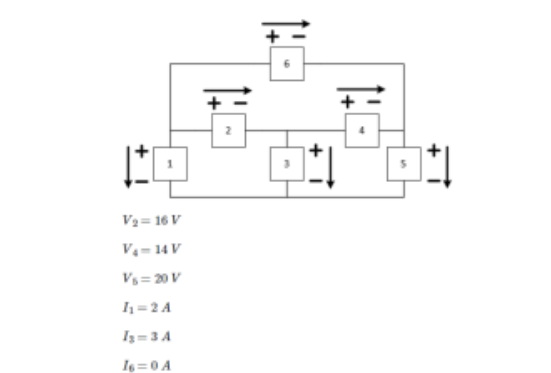
\includegraphics[width=0.75\linewidth]{figures/2.png}
\end{center}

\textbf{Question 5:} Given the above circuit and information, find V1, V3, V6, I2, I4, and I5.

\begin{center}
    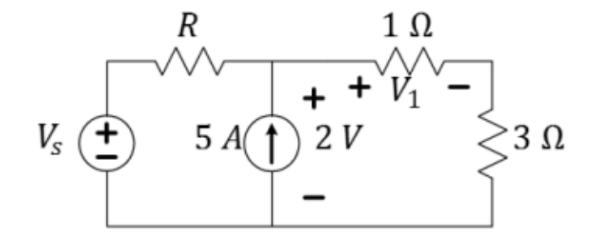
\includegraphics[width=0.75\linewidth]{figures/3.png}
\end{center}

\textbf{Question 6:} Find V1 in the above circuit.

\begin{center}

    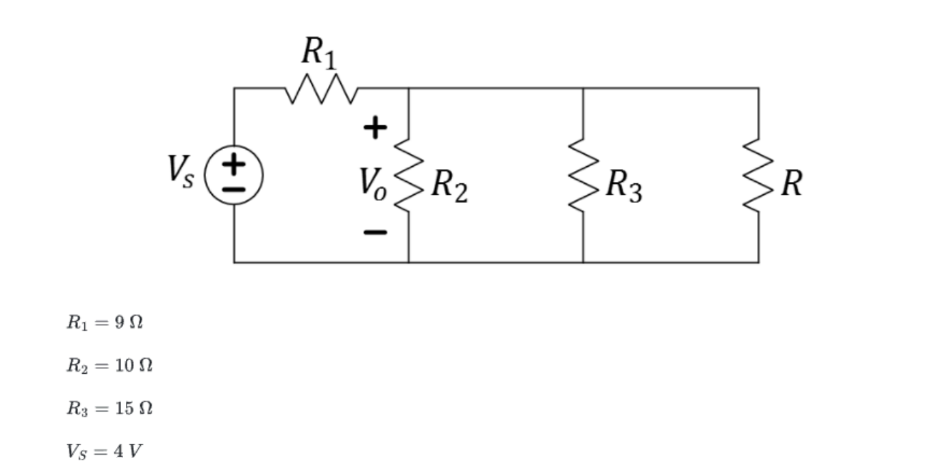
\includegraphics[width=0.75\linewidth]{figures/5.png}

\end{center}


\textbf{Question 7:} What value of R will result in Vo = 1V?

\begin{center}
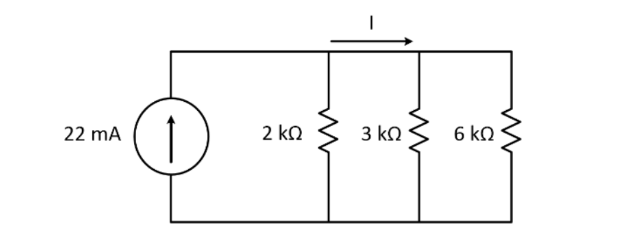
\includegraphics[width=0.75\linewidth]{figures/6.png}
\end{center}

\textbf{Question 8:} Find I in the above circuit.

\section*{Equivalent Resistance / Power}
\textbf{Question 9:} Find equivalent resistance for the circuits below.

\begin{center}

        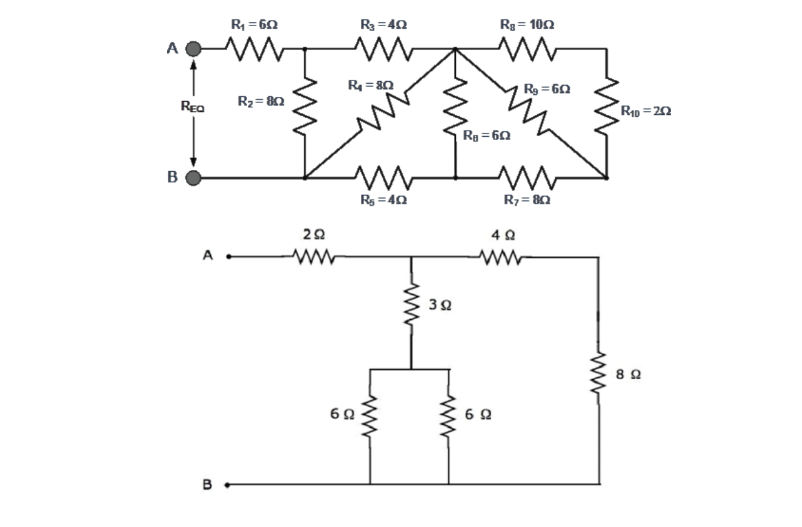
\includegraphics[width=0.75\linewidth]{figures/image.png}
\end{center}

\textbf{Question 10:} If the voltage between nodes A and B in the second circuit is 9V...
\begin{enumerate}
\item What is the current through the 3 ohm resistor?
\item What is the power through the 3 ohm resistor?
\item What is the power through the 8 ohm resistor?
\item What resistor has the highest power output?
\end{enumerate}

\section*{PWM}
\textbf{Question 11:} Imagine a square wave that outputs 15W from 0 to 12 seconds and 5W from 12 to 20 seconds. This square wave corresponds to a 10 ohm resistor.
\begin{enumerate}
    \item What is the Average Power of this waveform?
    \item What is the RMS Voltage of this waveform?
\end{enumerate}
\textbf{Question 12:} Given a limited portion of this graphed waveform, what is its duty cycle?

\begin{center}

        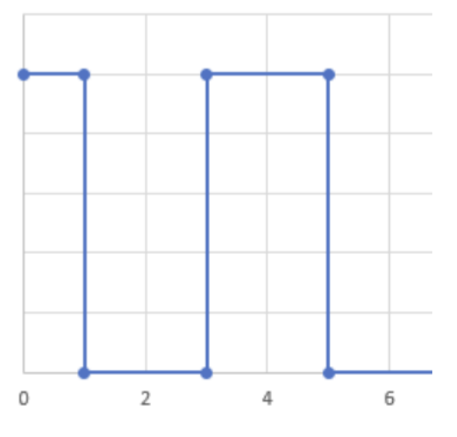
\includegraphics[width=0.75\linewidth]{figures/8.png}
\end{center}

\pagebreak

\section*{I-V Equations}
\textbf{Question 13:} What is the short circuit current and the open circuit voltage for the circuit below?
\begin{center}

        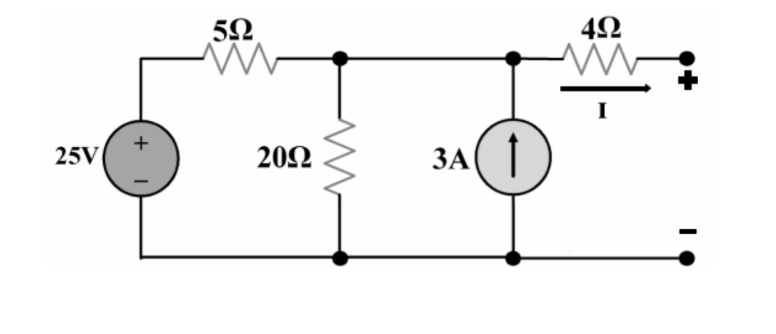
\includegraphics[width=0.75\linewidth]{figures/12.png}

\end{center}

\textbf{Question 14:} If this circuit were to be placed in series with another circuit with an IV equation of \(I = 0.005V - 0.025\), assuming the same polarities given above, what would be the operating current and voltage?

\textbf{Question 15:} If the open circuit voltage of a circuit containing ideal sources and resistors is measured at Voc = 8 V, while the current through the short circuit across the circuit is Isc = 200 mA, what would be the power in watts absorbed by an ideal voltage source, Vs = 4, placed across the terminals?

\begin{center}
    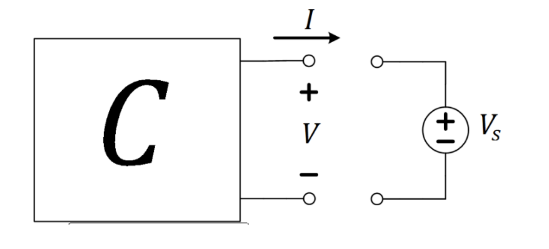
\includegraphics[width=0.75\linewidth]{figures/14.png}

\end{center}

\section*{Norton and Thevenin}
\textbf{Question 16:} Give Norton and Thevenin Forms for the subcircuit shown on the previous page.

\textbf{Question 17:} What is the Norton resistance of the circuit below? What is the Thevenin Resistance?

\textbf{Question 18:} Draw the Thevenin and Norton Equivalents.

\begin{center}
    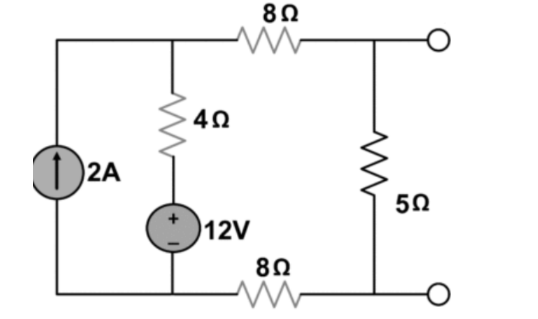
\includegraphics[width=0.75\linewidth]{figures/23.png}

\end{center}

\section*{Nodal Analysis}
\textbf{Question 19:} Find the voltage at node A for this circuit.

\textbf{Question 20:} Find the voltage drop across the 10, 30, and 50 ohm resistors.

\begin{center}
    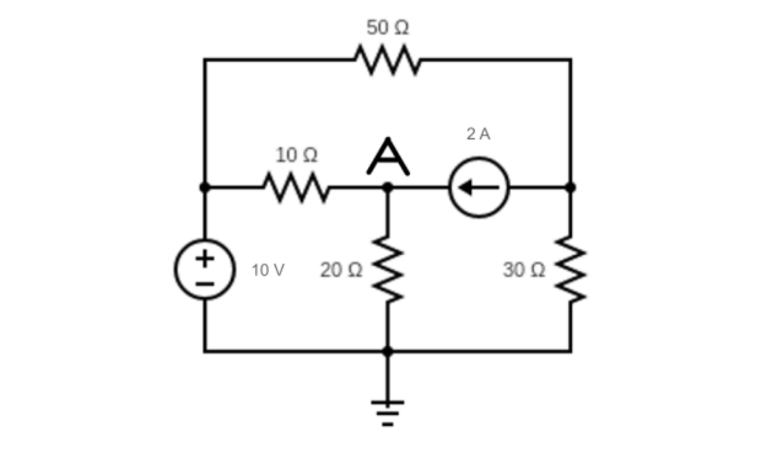
\includegraphics[width=0.75\linewidth]{figures/34.png}
\end{center}

\pagebreak

\section*{Diodes}
\textbf{Question 21:} Assume an ideal-offset model and Von = 1 volt. If Vs = 5 cos(\(\omega\)t) volts and V1 = 2 volts, what are the maximum and minimum voltages across the open nodes?

\begin{center}

        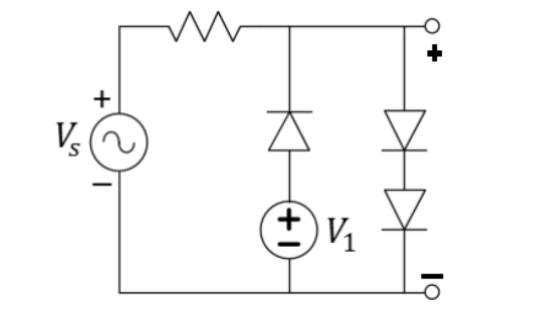
\includegraphics[width=0.75\linewidth]{figures/45.png}
\end{center}

\textbf{Question 22:} In the circuit below, which diodes are on? Furthermore, if Vs = 10 V, all the diodes have Von = 2V under the offset ideal model, and the voltage drop over R1 is also 2V, what is the voltage drop across the other resistors, assuming they have an equal resistance?

\begin{center}
    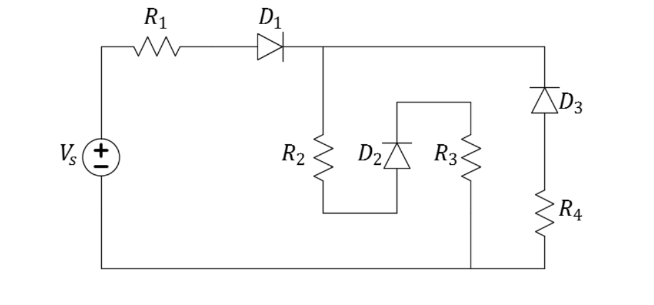
\includegraphics[width=0.75\linewidth]{figures/46.png}
\end{center}

\pagebreak

\section*{BJTs}
\textbf{Question 23:} The properties of the transistor are that VBE on is 1V, \(\beta\) is 120, and VCE sat is 0.2 V. In this circuit, VCC is 9V, RC is 150\(\Omega\), and RB is 30000\(\Omega\). What are the maximum and minimum values for VCE if Vi’s output is variable between 0V and 9V?

\begin{center}

    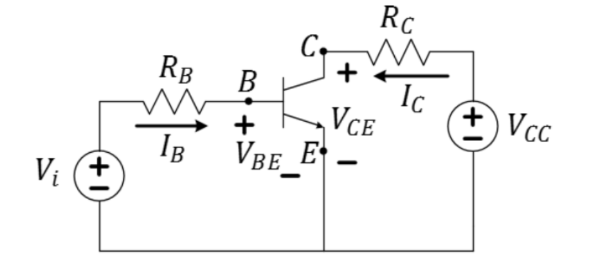
\includegraphics[width=0.75\linewidth]{figures/56.png}
\end{center}


\textbf{Question 24:} If Vi was set to 5V, what would VCE be?


\section*{MOSFETs/cMOS logic}
\textbf{Question 25:} An IC dissipates 110W. If the IC has a 5\% activity factor \(\alpha\), frequency of 10GHz, and 1nF gate capacitance, what is the maximum number of transistors that can be in the IC if it can operate at up to 9V?

\begin{center}

        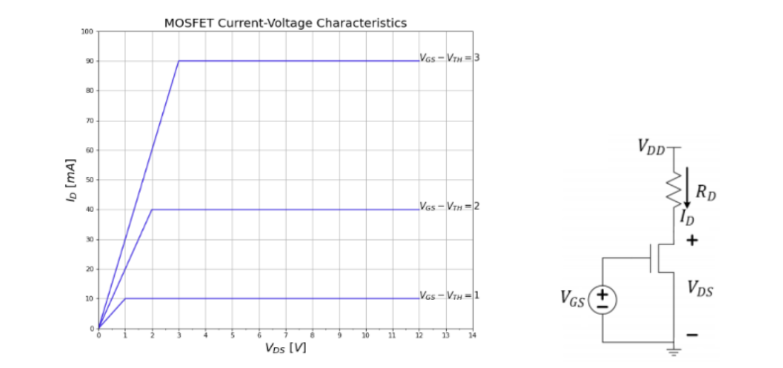
\includegraphics[width=1\linewidth]{figures/78.png}
\end{center}

\textbf{Question 26:} The given circuit with a MOSFET in series with a voltage source of 6V and a resistor with a resistance of 120\(\Omega\)
Find the transistor parameter k and a value for VDS that results in I = 30 mA, given that VGS - VTH = 2.

\section*{Bonus Questions}

\textbf{Question 27:} Give the IV equation, Norton equivalent, and Thevenin Equivalent for the circuit below.

\begin{center}

    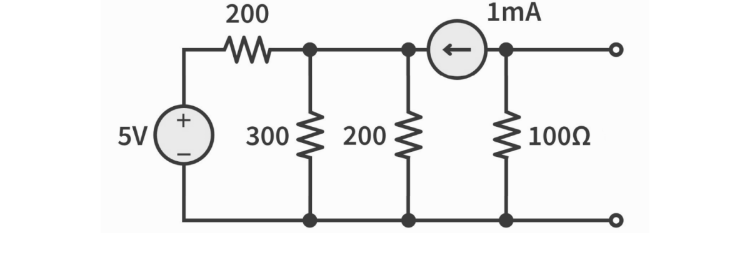
\includegraphics[width=0.75\linewidth]{figures/99.png}
\end{center}

\end{document}